\subsection{Experimental Results on STR-MF} \label{experimental_results_spatial}
Next we focus on using the Berkeley dataset to verify the STR-MF model because the traffic data does not contain sufficient location information to be exploited.

\begin{table} [htbp]
\caption{RMSE of Berkeley Random split} \label{table:spatial_random}
\setlength{\tabcolsep}{2pt}
\centering
\small
\begin{tabular} {c | r r r | r r r | r r r}
& \multicolumn{3}{ c|}{Humidity} & \multicolumn{3}{|c|}{Light} & \multicolumn{3}{|c }{Temperature} \\ \hline
train & \begin{turn}{65}TR-MF\end{turn} & \begin{turn}{65}STR-MF\end{turn} & \begin{turn}{65}sTR-MF\end{turn}& \begin{turn}{65}TR-MF\end{turn} & \begin{turn}{65}STR-MF\end{turn} & \begin{turn}{65}sTR-MF\end{turn}& \begin{turn}{65}TR-MF\end{turn} & \begin{turn}{65}STR-MF\end{turn} & \begin{turn}{65}sTR-MF\end{turn} \\ \hline
10\% & $ \mathbf{ 0.142 } $ & $ 0.484 $ & $ 0.173 $ & $ \mathbf{ 35.5 } $ & $ 97.4 $ & $ 38.3 $ & $ \mathbf{ 0.046 } $ & $ 0.154 $ & $ 0.061 $\\
20\% & $ \mathbf{ 0.114 } $ & $ 0.424 $ & $ 0.135 $ & $ \mathbf{ 28.2 } $ & $ 90.6 $ & $ 28.9 $ & $ \mathbf{ 0.032 } $ & $ 0.146 $ & $ 0.047 $\\
40\% & $ \mathbf{ 0.092 } $ & $ 0.352 $ & $ 0.104 $ & $ \mathbf{ 21.2 } $ & $ 85.8 $ & $ 22.8 $ & $ \mathbf{ 0.023 } $ & $ 0.145 $ & $ 0.037 $\\
60\% & $ \mathbf{ 0.082 } $ & $ 0.337 $ & $ 0.093 $ & $ \mathbf{ 17.2 } $ & $ 83.3 $ & $ 18.3 $ & $ \mathbf{ 0.018 } $ & $ 0.147 $ & $ 0.031 $\\
80\% & $ \mathbf{ 0.076 } $ & $ 0.324 $ & $ 0.084 $ & $ \mathbf{ 17.7 } $ & $ 84.4 $ & $ 18.1 $ & $ \mathbf{ 0.015 } $ & $ 0.148 $ & $ 0.027 $\\
85\% & $ \mathbf{ 0.075 } $ & $ 0.326 $ & $ 0.083 $ & $ \mathbf{ 14.4 } $ & $ 82.0 $ & $ 15.8 $ & $ \mathbf{ 0.016 } $ & $ 0.138 $ & $ 0.028 $\\
\end{tabular}
\end{table}

\begin{table} [htbp]
\caption{RMSE of Berkeley Temporal split} \label{table:spatial_temporal}
\setlength{\tabcolsep}{2pt}
\centering
\small
\begin{tabular} {c | r r r | r r r | r r r}
& \multicolumn{3}{ c|}{Humidity} & \multicolumn{3}{|c|}{Light} & \multicolumn{3}{|c }{Temperature} \\ \hline
train & \begin{turn}{65}TR-MF\end{turn} & \begin{turn}{65}STR-MF\end{turn} & \begin{turn}{65}sTR-MF\end{turn}& \begin{turn}{65}TR-MF\end{turn} & \begin{turn}{65}STR-MF\end{turn} & \begin{turn}{65}sTR-MF\end{turn}& \begin{turn}{65}TR-MF\end{turn} & \begin{turn}{65}STR-MF\end{turn} & \begin{turn}{65}sTR-MF\end{turn} \\ \hline
10\% & $ 0.957 $&$ 0.573 $&$ \mathbf{ 0.547 } $&$ \mathbf{ 220.070 } $&$ 281.607 $&$ 264.763 $&$ 0.515 $&$ \mathbf{ 0.242 } $&$ 0.307 $\\
20\% & $ 0.796 $&$ 0.657 $&$ \mathbf{ 0.459 } $&$ \mathbf{ 113.310 } $&$ 236.865 $&$ 230.054 $&$ 0.392 $&$ \mathbf{ 0.179 } $&$ 0.187 $\\
40\% & $ 0.771 $&$ 0.520 $&$ \mathbf{ 0.455 } $&$ \mathbf{ 58.090 } $  & $ 110.758 $ &  $ 64.388 $&$ 0.310 $&$ 0.196 $&$ \mathbf{ 0.189 } $\\
60\% & $ 0.540 $&$ \mathbf{ 0.351 } $&$ 0.708 $&$ \mathbf{ 41.730 } $  & $ 150.149 $ &  $ 69.235 $&$ 0.206 $&$ \mathbf{ 0.191 } $&$ 0.243 $\\
80\% & $ 0.447 $&$ 0.299 $&$ \mathbf{ 0.261 } $&$ \mathbf{ 21.450 } $  & $ 112.694 $ &  $ 28.017 $&$ 0.132 $&$ \mathbf{ 0.108 } $&$ 0.114 $\\
85\% & $ 0.323 $&$ \mathbf{ 0.166 } $&$ 0.256 $&$ \mathbf{ 8.310 } $   & $ 85.423 $  &  $ 12.079 $&$ 0.088 $&$ \mathbf{ 0.065 } $&$ 0.082 $\\
\end{tabular}
\end{table}



%Table \ref{table:spatial_random_hum}, \ref{table:spatial_random_light}, \ref{table:spatial_random_tem}, \ref{table:spatial_temporal_hum}, \ref{table:spatial_temporal_light}, \ref{table:spatial_temporal_tem}  show the result of adding spatial regularization.
Table \ref{table:spatial_random} and \ref{table:spatial_temporal} compare STR-MF with TR-MF. The spatial regularization we used for STR-MF was defined based on manually determined neighborhood nodes given the floor plan, as shown in Figure \ref{fig:expected_similarity}.
Note that the capital STR-MF stands for TR-MF plus strong spatial regularization, while the small sTR-MF represents weaker spatial-regularized TR-MF. The results show that for random missing pattern, adding spatial regularization indeed hurts the performance. It is because in random missing cases, the information is sufficient for TR-MF to learn the correlations between sensors, while enforcing similarity between near-by sensors can hurt the performance because the sensors might not be that correlated. On the other hand, in the consecutive missing cases, adding spatial regularization does show significant improvement on humidity and temperature readings. In a nutshell, comparing TR-MF with STR-MF, the former is a pure data-driven model while the later is slightly knowledge-driven. The experiments show that when we have sufficient data to learn the correlation between sensors, it is better to ignore the given knowledge because they might not be accurate; however, if the given data is not sufficient, incorporating the external spatial knowledge can be helpful.


We also conduct an interesting experiment to see whether the correlation learned by TR-MF in random missing cases does reflect our hypothesis of spatial correlation (i.e. Figure \ref{fig:expected_similarity}). For each of the humidity and light data, we first use the TR-MF model to learn the latent factors of each sensor node given random missing under 85\% training data. Based on the latent factors $\mathbf{q}$, we can then define the similarity between sensor nodes $n_i$ and $n_j$ as:
%\begin{equation*}
$\frac{q_{n_i}^T q_{n_j}}{max(||q_{n_i}||^2, ||q_{n_j}||^2)},$
%\end{equation*}
and we get the similarity graph as Figure \ref{fig:similarity}.
\begin{figure}[ftbp]
\centering
\subfigure[Expected Similarity]{
	\label{fig:expected_similarity}
	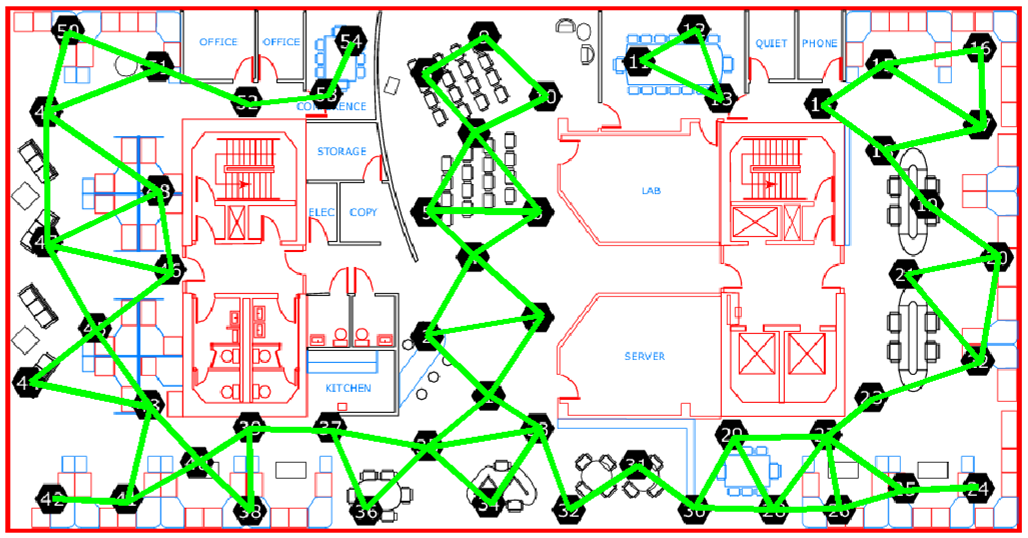
\includegraphics[width=0.25\textwidth]{expected.png}
}\\
\subfigure[Humidity: top 100 similar pairs]{
	\label{fig:humidity_similarity}
	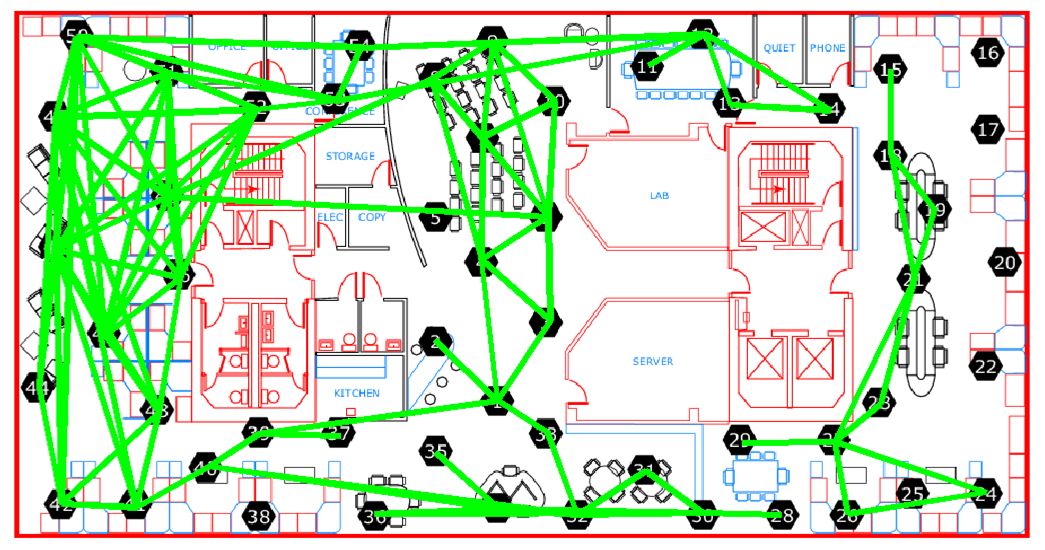
\includegraphics[width=0.22\textwidth]{Hum_similarity.png}
}
\hspace{0in}
\subfigure[Light: top 100 similar pairs]{
	\label{fig:light_similarity}
	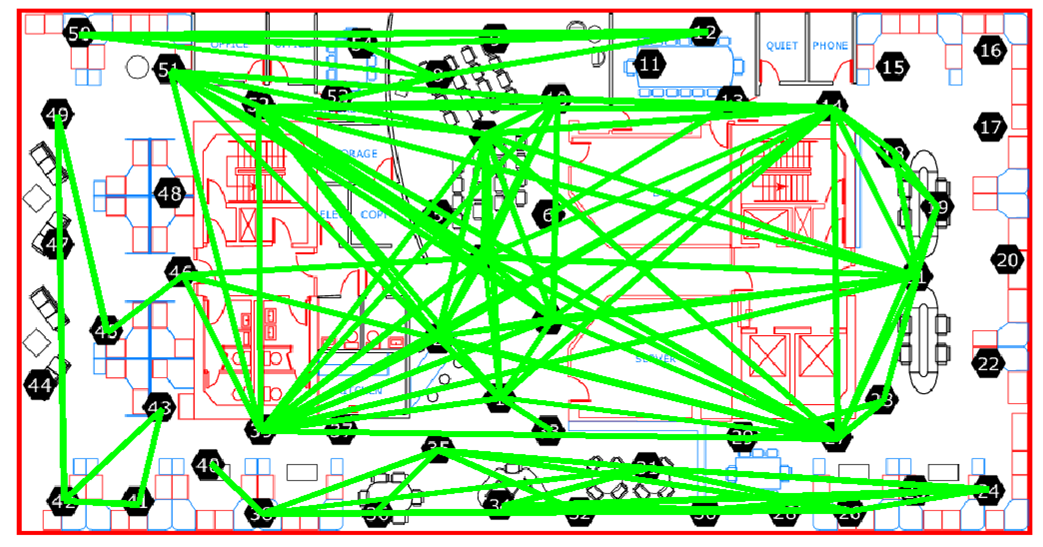
\includegraphics[width=0.22\textwidth]{Light_similarity.png}
}
\caption{similarity graph}
\label{fig:similarity}
\end{figure}

Then we identify the top 100 similar pairs and draw a line between each of them on the floor plan. We can see that the manually hypothesized spatial correlation plot Figure \ref{fig:expected_similarity} is more similar to the one learned from humidity data (Figure \ref{fig:humidity_similarity}) than to the one learned from light data (Figure \ref{fig:light_similarity}). This experiment shows two interesting insights. First, the manually crafted spatial correlation does not necessary reflect the true correlation between sensor signals, because they might have not yet considered other factors such as those described in the example of Figure \ref{fig:example_home_floorplan}. Second, if the human knowledge of spatial correlation does to some extent reflect the true correlation between sensors, incorporating them in scenarios with limited information (e.g. the consecutive missing pattens) can be helpful (i.e. the humidity imputation in Table \ref{table:spatial_temporal} improves with spatial information); otherwise it is useless (i.e. no improvement for the light imputation in Table \ref{table:spatial_temporal}).
